\title{\LaTeX Template}
\author{
        Kia Rahmani \\
                Department of Computer Science\\
        Purdue University, USA
}
\date{\today}

% Main Document
\documentclass[12pt,letter]{article}
\usepackage{xcolor,listings}
\usepackage{graphicx}
\usepackage[inline]{enumitem}
\usepackage[utf8]{inputenc}
\usepackage[english,ngerman]{babel}
\usepackage{amsmath}
\usepackage{mathtools}
\usepackage{mathpartir}

\begin{document}
\selectlanguage{english}
%\maketitle
%\begin{abstract} \end{abstract}


% Sections
% ---------------------------------------------------
\section{Description}
\paragraph{}
We have now added SER\footnote{Traditional fully isolated transactions}
transactions support on top of Quelea \cite{quelea}. The added mechanism uses an
external key-value database etcd\footnote{https://coreos.com/etcd/}
which implements the Raft consensus protocol to offer a high performance
distributed (but strongly consistent) store. I initially tried to use
Quelea's own SC operations to implement a simple locking mechanism. SC operations in Quelea are based on Cassandra's CAS
(compare and swap) lightweight transactions. However, implementation of CAS 
in Cassandra is very bad and show incorrect behavior even under light pressure
(and totally breaks down under congestion). 

In order to show the performance gain from  assigning 
fine-tuned  isolation guarantees to traditional SQL transactions, I
implemented a very simple version of TPC-C in Quelea. For this
experiment we did not need a full-fledged application with program logic
details to show the performance gain from weakly isolated transactions.
I created a set of simple transactions, according to TPC-C
specification, that work with Quelea's
LWW registers. The transacitons,  roughly follow the defined TPC-C behavior. For
example, our newOrder updates 6 registers each corresponding one task
from the original TPC-C. This has to be extended to a full programming
framework with an interesting enough logic, but for now, it suffices to
support our claims. The transactions are executed according to the
following table\footnote{The isolation levels are assigned following the
results in \cite{Bailis:2013:HAT}}:
\begin{center}
\begin{tabular}{ |l|c|c| } 
 \hline
 new order & SER & 5\% \\ 
 delivery  & SER & 40\% \\ 
 order status & MAV & 5\% \\ 
 payment & MAV & 45\% \\ 
 stock level & MAV & 5\% \\ 
 \hline
\end{tabular}
\end{center}

\section{Results}
The following results are from a 3-node amazon ec2 cluster running (Cassandra/Quelea + etcd). The cluster consists of t2.medium instances at Oregon, Ohio, and Virginia. 
Note that the extremely high latencies are due to the fact that 
all transactions are being coordinated since we are assuming a 
single object for now. This can be relaxed when we implement an object 
based lock and only coordinate transactions accessing the same object 
(e.g. in \cite{quelea} experiments are on objects that are randomly 
chosen from a set of 10000, which rarely causes any blocking).
The results show almost 50\% lower latency when using SER transactions only when they are absolutely needed:
\begin{figure}[h]
  \begin{center}
  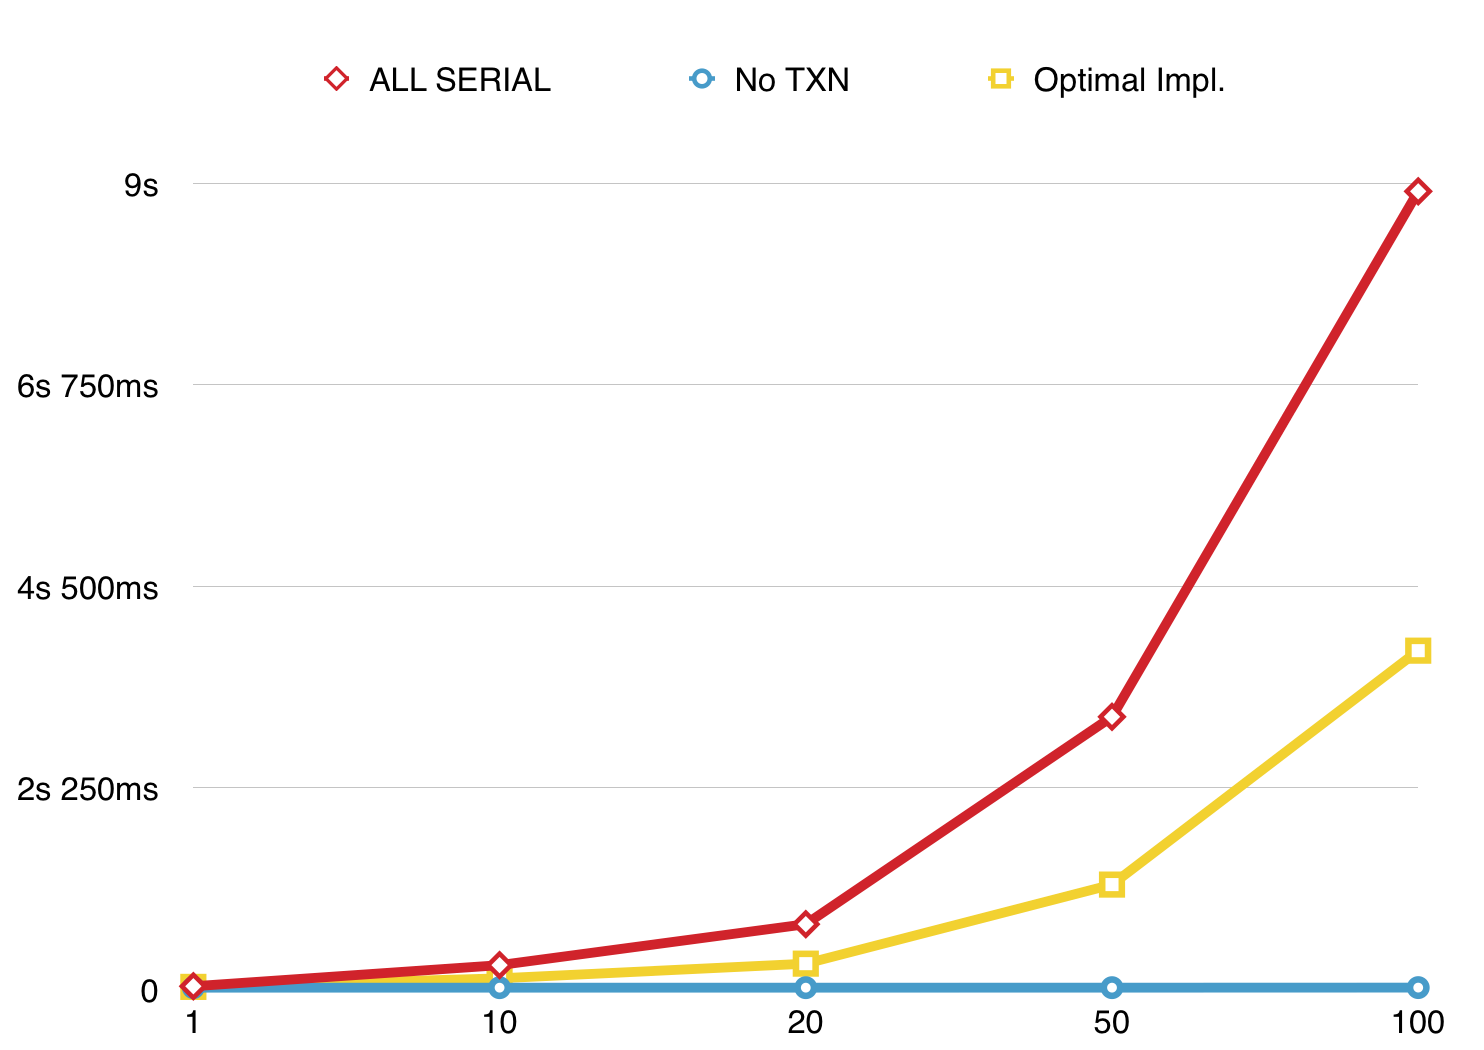
\includegraphics[width=0.9\textwidth]{figures/results.png}
  \end{center}
  \caption {Lantency vs number of concurrent clients}
\end{figure}

    




\section{To Do}
\begin{enumerate}
\item In the current lock implementation, clients try acquiring the lock and if they fail, they try again after 0.05 seconds. 
	Although this cannot affect the average latency of all
	operations (which we are measuring), but it can potentially cause starvation for some clients and should be extended to a fair locking system later. 
\item Currently, SER is implemented at the client side by acquiring a
	global lock. 
This task should be pushed into the server side in a more realistic system. 
We should also switch to an object-based lock to allow a higher through put.
\item Ultimately, we need a general purpose and full-fledged programming framework for writing EC applications on Quelea. 
The framework should be equal to L3 from the previous document.
\end{enumerate}








% The Biblography
\bibliographystyle{abbrv}
\bibliography{kia-bib}
\end{document}
